\documentclass[]{jarticle}          % 一段組
%\documentclass[twocolumn]{jarticle} % 二段組

\textwidth 180mm
\textheight 255mm
\oddsidemargin -12mm
\topmargin -15mm
\columnsep 10mm

%\vspace{0.5cm} % 一段組の場合はコメントアウトした方が体裁がよいx
%] % 一段組の場合はコメントアウトする

\usepackage{styles/labheadings}
\usepackage[dvipdfmx]{graphicx,color}
\usepackage{amsmath,amssymb}
\usepackage{url}
% 追加
\usepackage[hang,small,bf]{caption}
\usepackage[subrefformat=parens]{subcaption}
\captionsetup{compatibility=false}

\newcommand{\aU}{\mbox{\boldmath $a$}}
\newcommand{\bU}{\mbox{\boldmath $b$}}
\newcommand{\cU}{\mbox{\boldmath $c$}}
\newcommand{\dU}{\mbox{\boldmath $d$}}
\newcommand{\eU}{\mbox{\boldmath $e$}}
\newcommand{\fU}{\mbox{\boldmath $f$}}
\newcommand{\gU}{\mbox{\boldmath $g$}}
\newcommand{\hU}{\mbox{\boldmath $h$}}
\newcommand{\iU}{\mbox{\boldmath $i$}}
\newcommand{\jU}{\mbox{\boldmath $j$}}
\newcommand{\kU}{\mbox{\boldmath $k$}}
\newcommand{\lU}{\mbox{\boldmath $l$}}
\newcommand{\mU}{\mbox{\boldmath $m$}}
\newcommand{\nU}{\mbox{\boldmath $n$}}
\newcommand{\oU}{\mbox{\boldmath $o$}}
\newcommand{\pU}{\mbox{\boldmath $p$}}
\newcommand{\qU}{\mbox{\boldmath $q$}}
\newcommand{\rU}{\mbox{\boldmath $r$}}
\newcommand{\sU}{\mbox{\boldmath $s$}}
\newcommand{\tU}{\mbox{\boldmath $t$}}
\newcommand{\uU}{\mbox{\boldmath $u$}}
\newcommand{\vU}{\mbox{\boldmath $v$}}
\newcommand{\wU}{\mbox{\boldmath $w$}}
\newcommand{\xU}{\mbox{\boldmath $x$}}
\newcommand{\yU}{\mbox{\boldmath $y$}}
\newcommand{\zU}{\mbox{\boldmath $z$}}
\newcommand{\AU}{\mbox{\boldmath $A$}}
\newcommand{\BU}{\mbox{\boldmath $B$}}
\newcommand{\CU}{\mbox{\boldmath $C$}}
\newcommand{\DU}{\mbox{\boldmath $D$}}
\newcommand{\EU}{\mbox{\boldmath $E$}}
\newcommand{\FU}{\mbox{\boldmath $F$}}
\newcommand{\GU}{\mbox{\boldmath $G$}}
\newcommand{\HU}{\mbox{\boldmath $H$}}
\newcommand{\IU}{\mbox{\boldmath $I$}}
\newcommand{\JU}{\mbox{\boldmath $J$}}
\newcommand{\KU}{\mbox{\boldmath $K$}}
\newcommand{\LU}{\mbox{\boldmath $L$}}
\newcommand{\MU}{\mbox{\boldmath $M$}}
\newcommand{\NU}{\mbox{\boldmath $N$}}
\newcommand{\OU}{\mbox{\boldmath $O$}}
\newcommand{\PU}{\mbox{\boldmath $P$}}
\newcommand{\QU}{\mbox{\boldmath $Q$}}
\newcommand{\RU}{\mbox{\boldmath $R$}}
\newcommand{\SU}{\mbox{\boldmath $S$}}
\newcommand{\TU}{\mbox{\boldmath $T$}}
\newcommand{\UU}{\mbox{\boldmath $U$}}
\newcommand{\VU}{\mbox{\boldmath $V$}}
\newcommand{\WU}{\mbox{\boldmath $W$}}
\newcommand{\XU}{\mbox{\boldmath $X$}}
\newcommand{\YU}{\mbox{\boldmath $Y$}}
\newcommand{\ZU}{\mbox{\boldmath $Z$}}
\newcommand{\epU}{\mbox{\boldmath $\epsilon$}}
\newcommand{\taU}{\mbox{\boldmath $\tau$}}
\newcommand{\etU}{\mbox{\boldmath $\eta$}}
\newcommand{\xiU}{\mbox{\boldmath $\xi$}}
\newcommand{\wwU}{\mbox{\boldmath $\omega$}}
\newcommand{\WwU}{\mbox{\boldmath $\Omega$}}
\newcommand{\lmU}{\mbox{\boldmath $\lambda$}}
\newcommand{\LmU}{\mbox{\boldmath $\Lambda$}}
\newcommand{\PiU}{\mbox{\boldmath $\Pi$}}
\newcommand{\SgU}{\mbox{\boldmath $\Sigma$}}
\newcommand{\thU}{\mbox{\boldmath $\theta$}}
\newcommand{\ThU}{\mbox{\boldmath $\Theta$}}
\newcommand{\roU}{\mbox{\boldmath $\rho$}}
\newcommand{\nuU}{\mbox{\boldmath $\nu$}}
\newcommand{\ones}{{\bf 1}}
\newcommand{\zr}{{\bf 0}}
\newcommand{\eq}{\begin{equation}}
\newcommand{\en}{\end{equation}}
\newcommand{\eqa}{\begin{eqnarray}}
\newcommand{\ena}{\end{eqnarray}}
\newcommand{\xx}{\makebox[1cm]{}}
\newcommand{\xm}{\makebox[0.5cm]{}}
\newcommand{\x}{\makebox[0.2cm]{}}
\newcommand{\tr}{{\rm tr}}
\newcommand{\sgn}{{\rm sgn}}
\newcommand{\ad}{{\rm ad}}

\newcommand{\rank}{{\rm rank}}
\newcommand{\diag}{{\rm diag}}
\newcommand{\lbr}{\left(\begin{array}}
\newcommand{\rbr}{\end{array}\right)}
\newcommand{\Proof}{\noindent{\em Proof\/}}
\newcommand{\Solution}{\noindent{\em Solution}}
\newcommand{\Derivation}{\noindent{\em Derivation}}
\newcommand{\msp}{\vspace*{\medskipamount}\\}
\newcommand{\qed}{\hspace*{\fill}$\Box$}
\newcommand{\aX}{{\bf a}}
\newcommand{\bX}{{\bf b}}
\newcommand{\cX}{{\bf c}}
\newcommand{\dX}{{\bf d}}
\newcommand{\eX}{{\bf e}}
\newcommand{\fX}{{\bf f}}
\newcommand{\gX}{{\bf g}}
\newcommand{\hX}{{\bf h}}
\newcommand{\iX}{{\bf i}}
\newcommand{\jX}{{\bf j}}
\newcommand{\kX}{{\bf k}}
\newcommand{\lX}{{\bf l}}
\newcommand{\mX}{{\bf m}}
\newcommand{\nX}{{\bf n}}
\newcommand{\oX}{{\bf o}}
\newcommand{\pX}{{\bf p}}
\newcommand{\qX}{{\bf q}}
\newcommand{\rX}{{\bf r}}
\newcommand{\sX}{{\bf s}}
\newcommand{\tX}{{\bf t}}
\newcommand{\uX}{{\bf u}}
\newcommand{\vX}{{\bf v}}
\newcommand{\wX}{{\bf w}}
\newcommand{\xX}{{\bf x}}
\newcommand{\yX}{{\bf y}}
\newcommand{\zX}{{\bf z}}
\newcommand{\AX}{{\bf A}}
\newcommand{\BX}{{\bf B}}
\newcommand{\CX}{{\bf C}}
\newcommand{\DX}{{\bf D}}
\newcommand{\EX}{{\bf E}}
\newcommand{\FX}{{\bf F}}
\newcommand{\GX}{{\bf G}}
\newcommand{\HX}{{\bf H}}
\newcommand{\IX}{{\bf I}}
\newcommand{\JX}{{\bf J}}
\newcommand{\KX}{{\bf K}}
\newcommand{\LX}{{\bf L}}
\newcommand{\MX}{{\bf M}}
\newcommand{\NX}{{\bf N}}
\newcommand{\OX}{{\bf O}}
\newcommand{\PX}{{\bf P}}
\newcommand{\QX}{{\bf Q}}
\newcommand{\RX}{{\bf R}}
\newcommand{\SX}{{\bf S}}
\newcommand{\TX}{{\bf T}}
\newcommand{\UX}{{\bf U}}
\newcommand{\VX}{{\bf V}}
\newcommand{\WX}{{\bf W}}
\newcommand{\XX}{{\bf X}}
\newcommand{\YX}{{\bf Y}}
\newcommand{\ZX}{{\bf Z}}

% report.texと同じディレクトリにnumerical_definition.texを入れておけば上の書き方でもいいはずです

\usepackage[
  dvipdfm,
  bookmarks=true,
  bookmarksnumbered=true,
  colorlinks=true]{hyperref}
\AtBeginDvi{\special{pdf:tounicode EUC-UCS2}}

\pagestyle{labheadings}
\headerleft{2次元フロアマップからのシーンの3次元モデルの作成}   % ヘッダの左側のタイトル
\headerright{2024年6月28日}  % ヘッダの右側のタイトル

\begin{document}

%\twocolumn % 一段組の場合はコメントアウトする

\vspace*{2ex}
\begin{center}
 {\Large \bf 3次元モデルに対するテクスチャ貼り付け}\\ % タイトル
 \vspace*{5mm}
 {\large M1 田川幸汰}% 発表者名
\end{center}

%\vspace{0.5cm} % 一段組の場合はコメントアウトした方が体裁がよいx
%] % 一段組の場合はコメントアウトする

%新しく作成したコマンド
% \newcommand{\reffig}[1]{\hyperref[#1]{図\ref{#1}}}
% \newcommand{\refeq}[1]{\hyperref[#1]{式(\ref{#1})}}
% \newcommand{\reftab}[1]{\hyperref[#1]{表\ref{#1}}}
% \newcommand{\refsec}[1]{\hyperref[#1]{\ref{#1}章}}
% \newcommand{\refsubsec}[1]{\hyperref[#1]{\ref{#1}節}}

% 数式
%\begin{equation}
%  数式記述  
%  \label{ラベル名}
%\end{equation}

% 図
% \begin{figure}[!ht]
%   \begin{center}
%     \includegraphics[scale=0.5]{figures/画像ファイル名}
%     \caption{キャプション名}
%     \label{ラベル名}
%   \end{center}
% \end{figure}

% リスト
% \begin{enumerate or itemize}
%   \item 
% \end{enumerate or itemize}
\section{テクスチャの取得}
\subsection{テクスチャ取得手法}
3次元モデルに対して正しい大きさ、位置、方向でテクスチャを割り当てる。
メッシュの重心に対してカメラの視線を向けるように作成した透視投影画像からテクスチャを取得する。
テクスチャを取得する具体的な手順を下に示す\cite{bib_1}。
\begin{enumerate}
  \item メッシュを構成する3点をカメラの外部パラメータを用いて世界座標系からカメラ座標系に変換する。
  \item メッシュ重心座標を計算する。
  \item カメラ中心から重心座標までの距離がしきい値以内のメッシュに対して以下の処理を行う。
  \item メッシュの法線ベクトルを計算する。
  \item カメラ中心から重心に向かうベクトルとメッシュの法線ベクトルとのなす角度がしきい値以内のメッシュに対して以下の処理を行う。
  \item カメラの視線が重心ベクトルを向くような回転行列を計算し、三角形メッシュの座標を変換する。
  \item カメラの内部パラメータを用いて三角形メッシュの座標を画像面上に投影する。
  \item メッシュを構成する3点が画像面上に収まっている場合、全方位画像から透視投影画像を作成する。
\end{enumerate}

ただし、全方位画像から透視投影画像を作成するにあたって、
前回の進捗報告で示した、直行射影の共線性と共面性を用いたカメラ姿勢推定の結果を用いたが、
正しい透視投影画像を得ることができなかった。
この原因として、自分が実装したテクスチャ生成のプログラムとカメラパラメータのどちらかに問題があると考え、
カメラパラメータとして真値を用いることで、プログラムが正しく動いているか検証した。

テクスチャ生成に使用した全方位カメラの内部パラメータ行列$\CU$を以下に示す。
$f_x,f_y$はカメラの焦点距離、$c_x,c_y$は光軸中心を表す。
\begin{equation}
  \CU = 
  \begin{pmatrix}
    f_x & 0 & c_x \\
    0 & f_y & c_y \\
    0 & 0 & 1 \\
  \end{pmatrix}
  =
  \begin{pmatrix}
    1000 & 0 & 800 \\
    0 & 1000 & 450 \\
    0 & 0 & 1 \\
  \end{pmatrix}
\end{equation}
また、カメラの外部パラメータである、回転行列$\RU$、並進ベクトル$\tU$を以下に示す。
\begin{equation}
  \RU = 
  \begin{pmatrix}
    1 & 0 & 0 \\
    0 & 0 & -1 \\
    0 & 1 & 0 \\
  \end{pmatrix}
  ,
  \tU =
  \begin{pmatrix}
    -1.0 \\
    1.5 \\
    0 \\
  \end{pmatrix}
\end{equation}


\subsection{テクスチャ作成結果}
入力として用いた全方位画像を\hyperref[two]{図\ref{two}}に示す。
\begin{figure}[!ht]
  \begin{center}
    \begin{tabular}{c}
      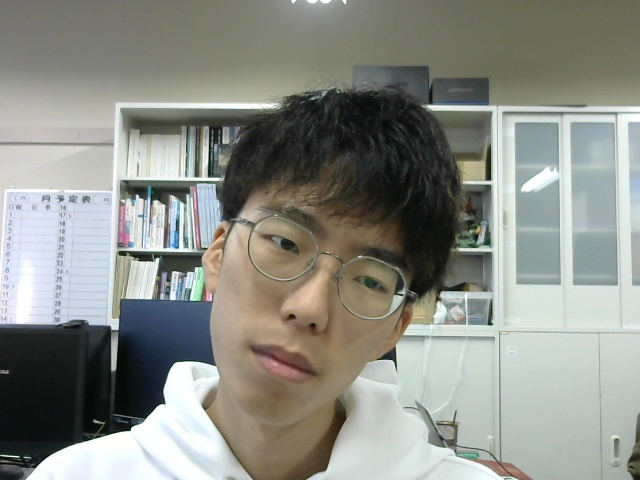
\includegraphics[keepaspectratio,  width=0.7\linewidth]{figures/texture.jpg}
    \end{tabular}
  \end{center}
  \caption{全方位画像}
  \label{two}
\end{figure}

\newpage

作成されたテクスチャの一部を\hyperref[three]{図\ref{three}}に示す。
ここで、赤の点は座標変換後のメッシュを構成する3点である。

\begin{figure}[!ht]
  \begin{center}
    \begin{tabular}{cc}
      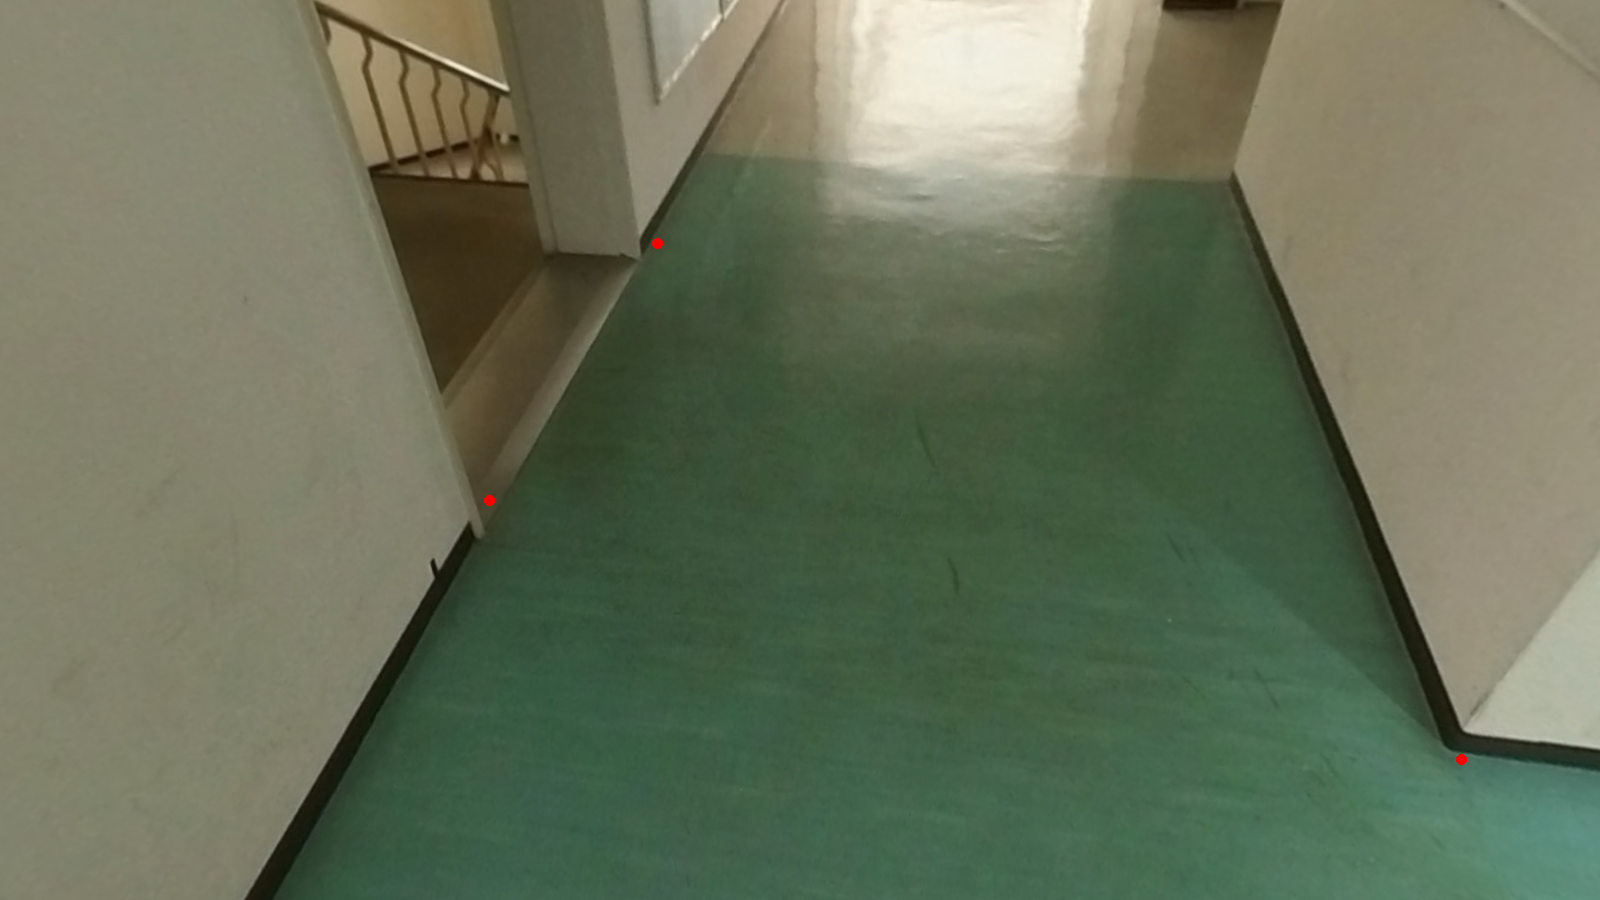
\includegraphics[keepaspectratio, width=0.4\linewidth]{figures/result/texture_1_1.png}&
      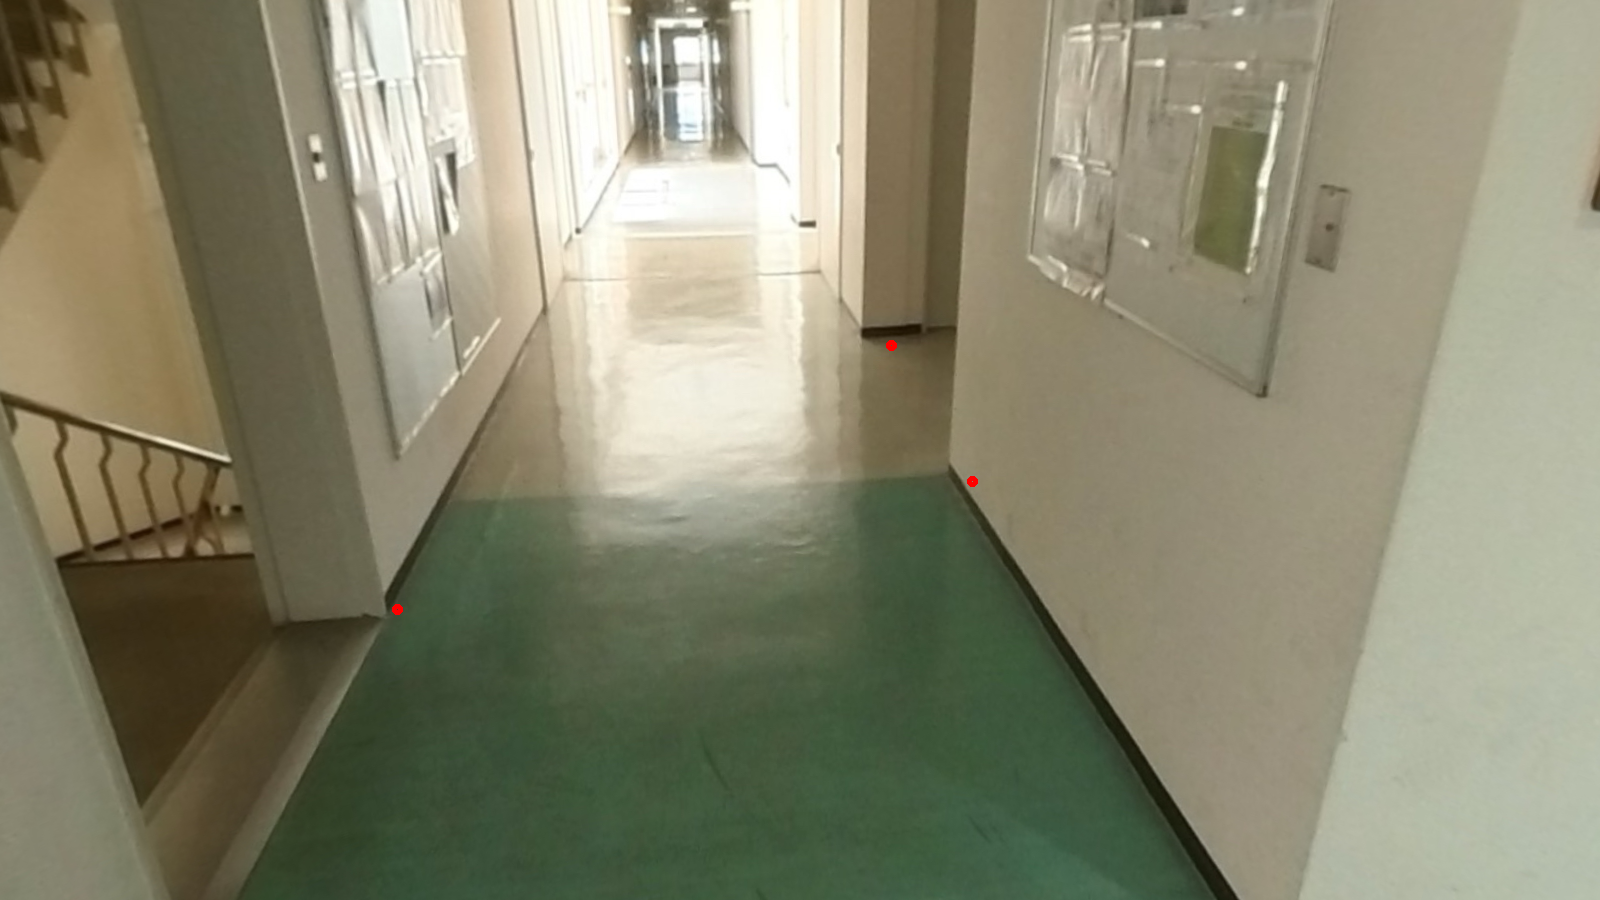
\includegraphics[keepaspectratio, width=0.4\linewidth]{figures/result/texture_1_3.png}\\
      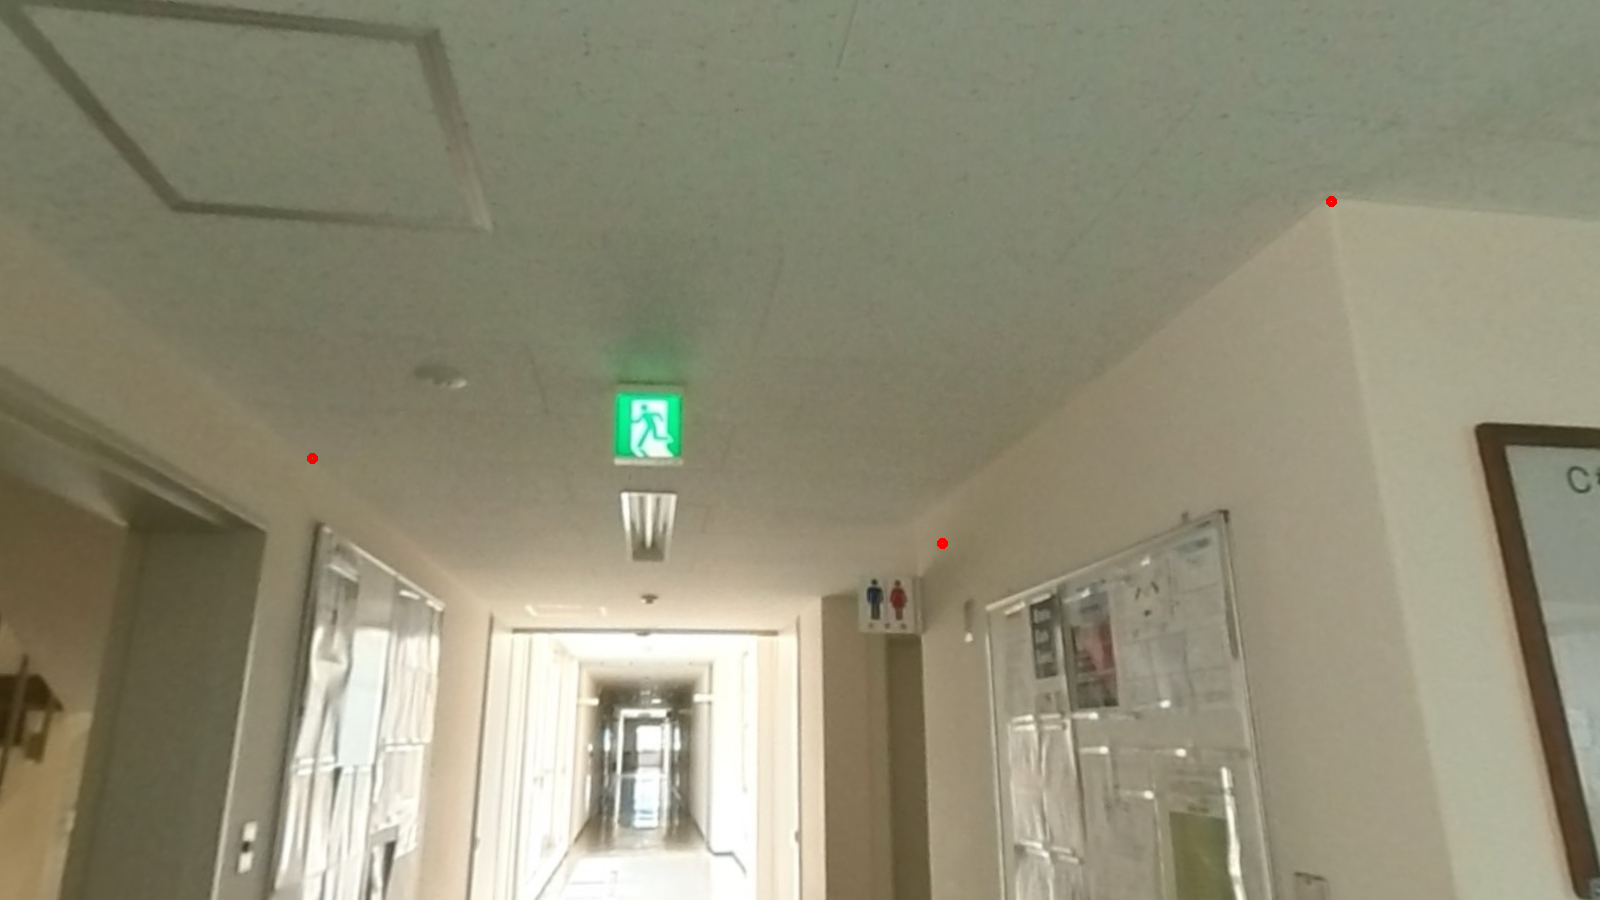
\includegraphics[keepaspectratio, width=0.4\linewidth]{figures/result/texture_1_5.png}&
      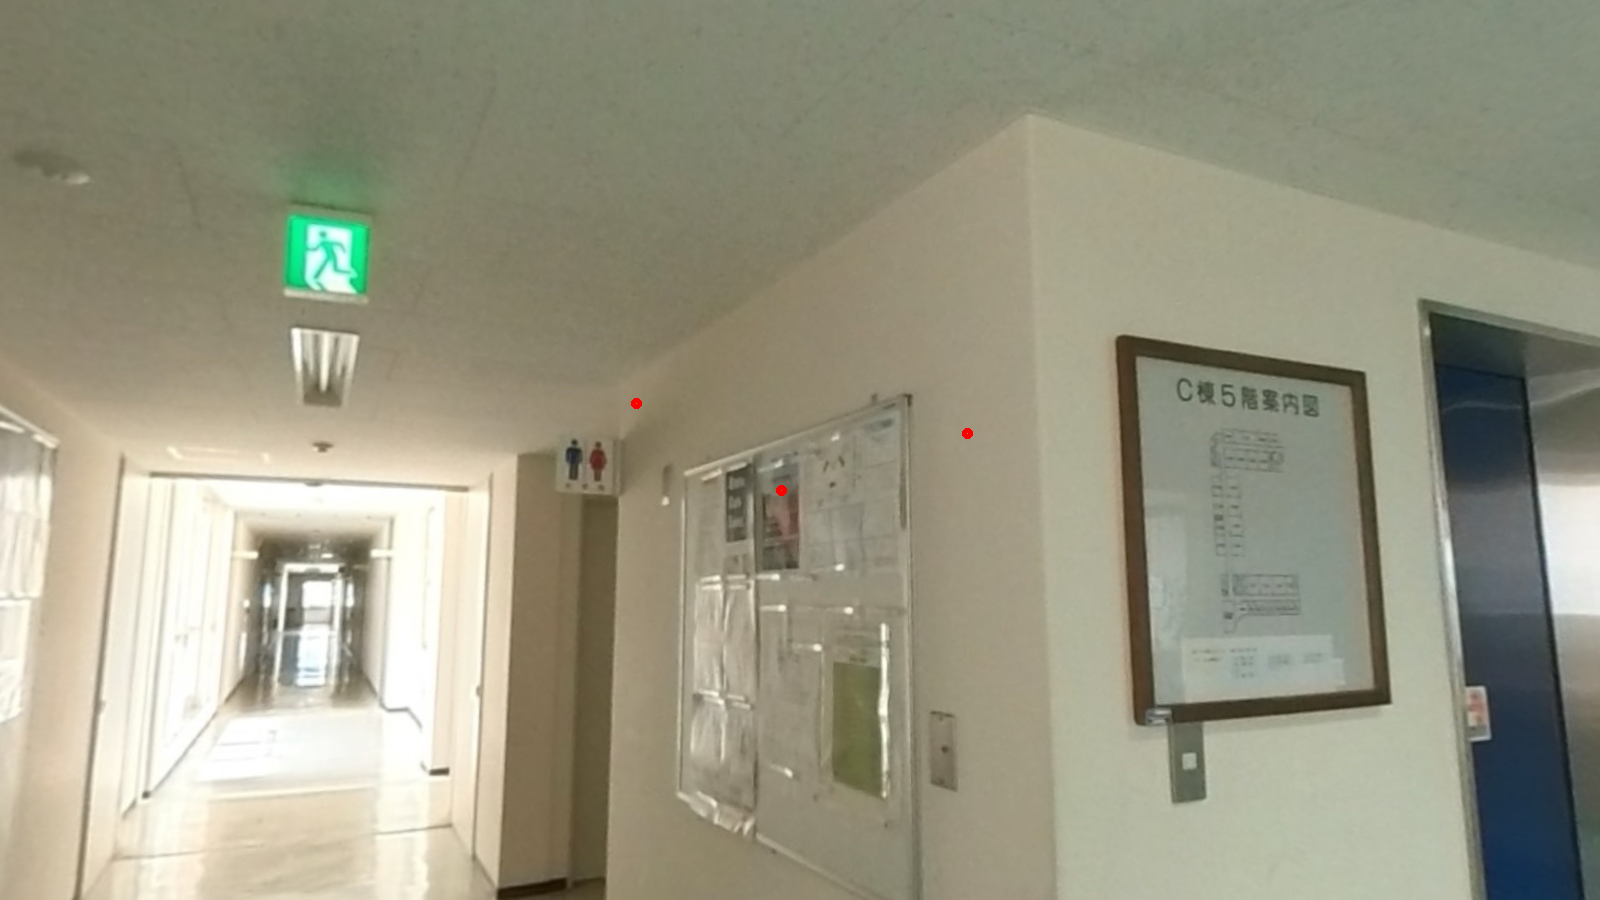
\includegraphics[keepaspectratio, width=0.4\linewidth]{figures/result/texture_1_7.png}\\
    \end{tabular}
  \end{center}
  \caption{テクスチャ取得結果}
  \label{three}
\end{figure}

床面のテクスチャについてはメッシュを構成する3点がかなり正しい位置に表示されている。
天井面のテクスチャについては少しずれてしまっているが、カメラ撮影の際に全方位カメラが傾いてしまったこと、
撮影位置が少しずれてしまったことで、カメラの外部パラメータが完全に正確ではなくなってしまったことが原因だと考えられる。
パラメータとして真値に近い値を用いたことで、大きな誤差はなくテクスチャが取得できてるようになったことから、
テクスチャ生成のプログラムは正しく動作していて、カメラパラメータ推定方法に何らかの問題があることがわかった。
また右下の図は、本来奥の天井面のテクスチャを取得しようとしているが、手前の壁のテクスチャを取得してしまっている。
本来取得したいテクスチャとカメラとの間に障害物がある場合は、取得しないようにするか別の全方位画像から得られたテクスチャに上書きする処理が必要であることがわかった。

\section{3次元モデルの作成}
透視投影画像と、画像面上に投影した座標を0~1の範囲で正規化したuv座標を用いて、3次元モデルにテクスチャを割り当てる。
3次元モデルファイルを書き換えてメッシュにテクスチャを割り当てた結果を\hyperref[four]{図\ref{four}}に示す。ここで、単色のテクスチャはデフォルトのテクスチャである。
左の画像は3次元モデルを前方から、右の画像は3次元モデルを上方から見た様子である。3次元モデルにテクスチャを割り当てることができていることがわかる。
\begin{figure}[!ht]
  \begin{center}
    \begin{tabular}{cc}
      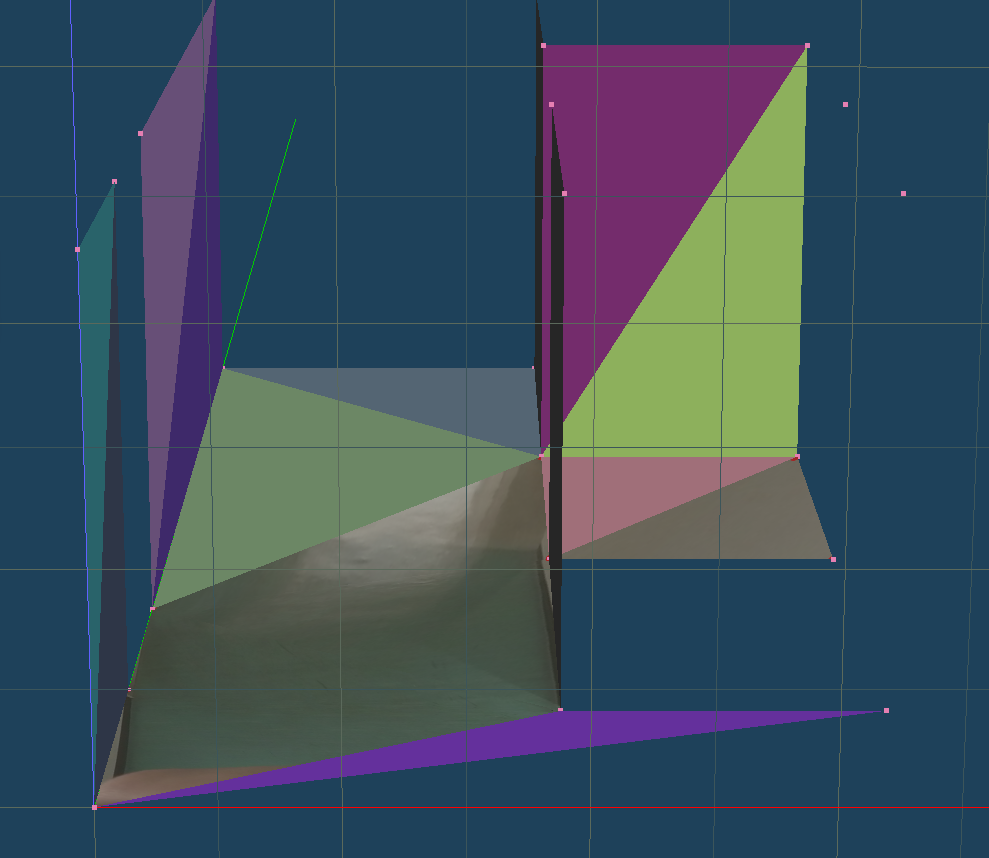
\includegraphics[keepaspectratio, width=0.4\linewidth]{figures/3dmodel0.png}&
      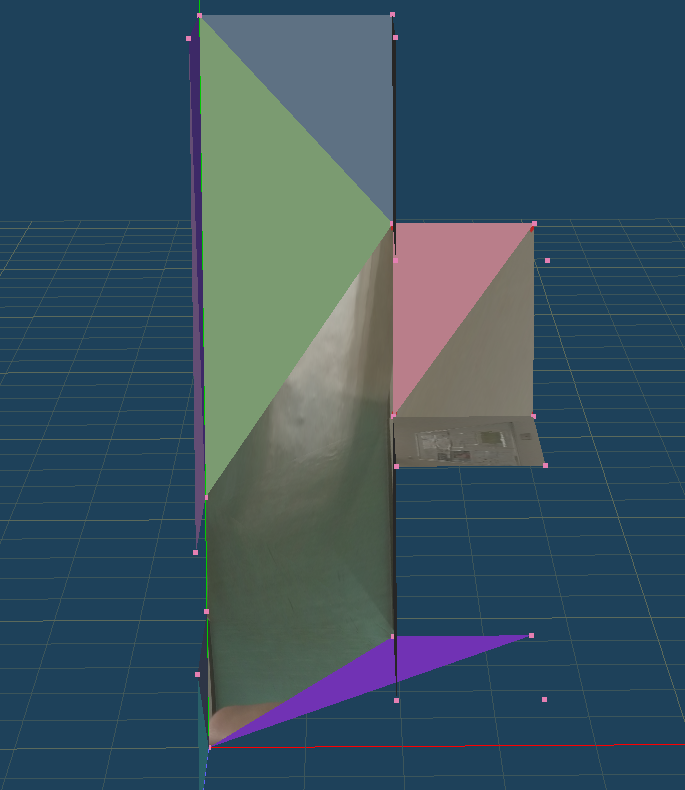
\includegraphics[keepaspectratio, width=0.4\linewidth]{figures/3dmodel1.png}\\
    \end{tabular}
  \end{center}
  \caption{3次元モデル}
  \label{four}
\end{figure}

\section{今後の計画}
カメラパラメータを真値ではなく、手動で推定して実際にテクスチャを取得する。
カメラ姿勢推定の誤差はどれくらい許容できるか、
また許容できないくらいの精度の場合どのようにして適切なテクスチャを得るか、カメラ姿勢推定精度の向上以外のアプローチについて考える。
具体的には、カメラ位置を移動して複数の全方位画像を用いることで、より良いテクスチャを取得することから進めていくつもりである。
%参考文献
\begin{thebibliography}{99}
\bibitem{bib_1} 菅谷保之,「3次元モデルへのテクスチャ貼付け」, 2024年7月17日閲覧.
\end{thebibliography}

\end{document}
